\chapter{РАЗРАБОТКА СИСТЕМЫ ПО ОПРЕДЕЛЕНИЮ ПОЗ СОБАК ПО ВИДЕО}

\section{Обучение нейронной сети} \label {second_iter}

В литературном обзоре было указано несколько архитектур нейронных сетей, которые предназначены для классификации изображений. В таблице \ref{tab:arch_comparison} приведена сравнительная точность таких архитектур на полученном датасете.

\begin{table}[H]
    \centering
    \captionsetup{justification=centering}
    \caption{\label{tab:arch_comparison} Сравнение точности разных архитектур компьютерного зрения и человека}
    \begin{tabularx}{\textwidth}{| Y | Y |}\hline
    Архитектура     & Точность \\\hline
    ResNet-50       &   80\%    \\\hline
    MobileNetV2     &   96\%    \\\hline
    Google's Visual Transformer   &     87\%\\\hline
    OpenAI CLIP     &   76\%    \\\hline
    Человек         &   98\%    \\\hline
    \end{tabularx}
\end{table}



Для того, чтобы получить наилучшие результаты классификации, было применено множество хорошо зарекомендовавших себя техник.

\subsection{Кадрирование с помощью нейронных сетей}
Одна из них -- это предварительная обрезка изображений нейронной сетью для сегментации изображений. Для этого использовалась предобученная MaskRCNN \cite{maskrcnn}.  Она получает на вход изображение $I$ и возвращает маску объектов $M$, находящихся на ней.

Маска -- это бинарное изображение, по высоте и ширине совпадающее с входным изображением, где наличие сигнала (белый цвет) говорит о наличии объекта на кадре. Наглядно это показано на рисунке \ref{img:mask}.
\begin{figure}[ht] 
  \centering
  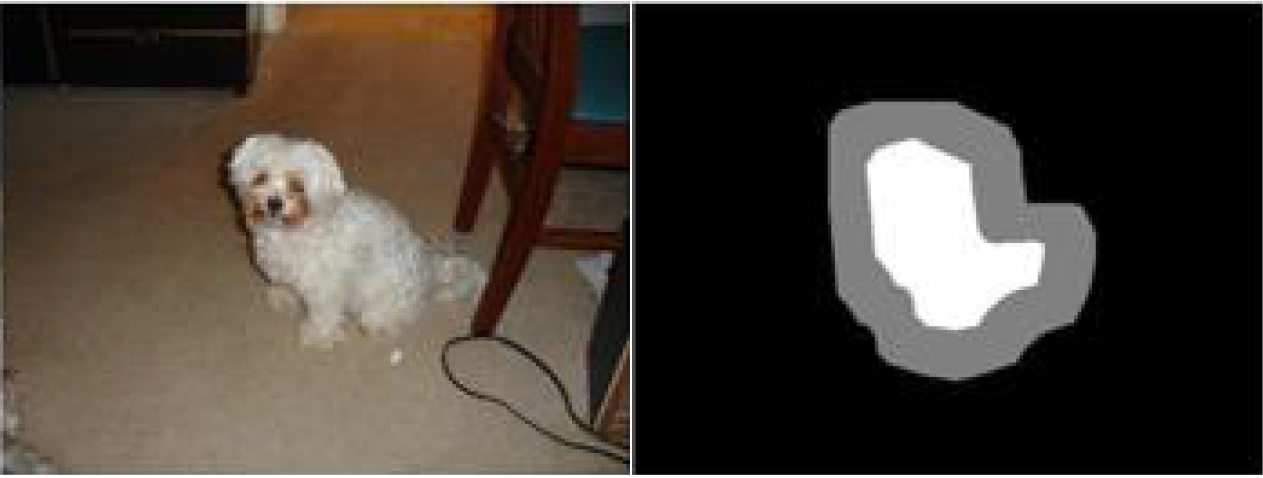
\includegraphics [width=\textwidth*2/3] {mask}
  \caption{Изображение собаки и маска собаки для этого изображения} 
  \label{img:mask}  
\end{figure}

Если на маске собаки несколько замкнутых фигур, значит, на кадре больше одной собаки и такое изображение использовать нельзя и необходимо разделить. Эти простые проверки сильно увеличивают качество обучающих данных для нейронной сети.

\subsection{Предобучение нейронной сети}
Другая техника для улучшения качества предсказаний - это предобучение нейронной сети. Обучающий массив в 4500 тысячи изображений является лишь условно достаточным для обучения таких крупных нейронных сетей как ResNet-50 и даже MobileNet. Поэтому такие нейронные сети всегда предобучают на больших наборах данных чтобы нейронная сеть лучше понимала какие изображения в принципе бывают. В данном случае используются нейронные сети, предобученные на ImageNet. После обучения на ImageNet, "голова" классификации заменяется на новую и обучается на новом наборе данных. При этом, свёрточные слои остаются нетронутыми. Такой подход называется в литературе Transfer Learning. Похожим принципом были обучены и остальные архитектуры, приведённные в таблице \ref{tab:arch_comparison}, но из-за ограничений в производительности была выбрана MobileNetV2. О ней и будет сказано далее.

\subsection{Характеристики полученной нейронной сети}
Характеристики полученной нейронной сети следующие:

\begin{itemize}[wide]
    \item Входное изображение I обладает размерностью 96 пикселей по ширине и высоте и 3 цветовыми каналами;
    \item Свёрточные слои нейронной сети MobileNet V2\cite{mobilenet}, без "головы";
    \item Global Average Pooling - последняя карта активации(3-мерный тензор $T$ с размерностью $\{x_{d1}, y_{d2}, z_{d3}\}$) преобразуется в плоский вектор $X$ с длинной $d_3$. Каждый слой превращается в одно число - среднее по слою. Это позволяет нейронной сети быть инвариантной к размеру входного изображения;
    
    \begin{equation}
    X_i = \dfrac{1}{d_1*d_2}\sum_{j=0}^{j=d_1}\sum_{k=0}^{k=d_2}T_{i,j,k}
    \end{equation}
    
    \item Слой DropOut\cite{dropout} - обнуление 20\% разных значений предыдущего слоя;
    \item Batch Norm\cite{batchnorm} - нормализация вектора относительно других изображений в мини-партии данных для обучения;
    \item Полносвязный слой с 512 нейронами;
    \item Функция активации, ReLU;
    \item слой DropOut;
    \item BatchNorm;
    \item Выходной слой $n$ нейронов, по количеству классов. Функция активации softmax.
\end{itemize}
Визуально архитектура представлена на рисунке \ref{img:NN_arch}.

\begin{figure}[ht] 
  \center
  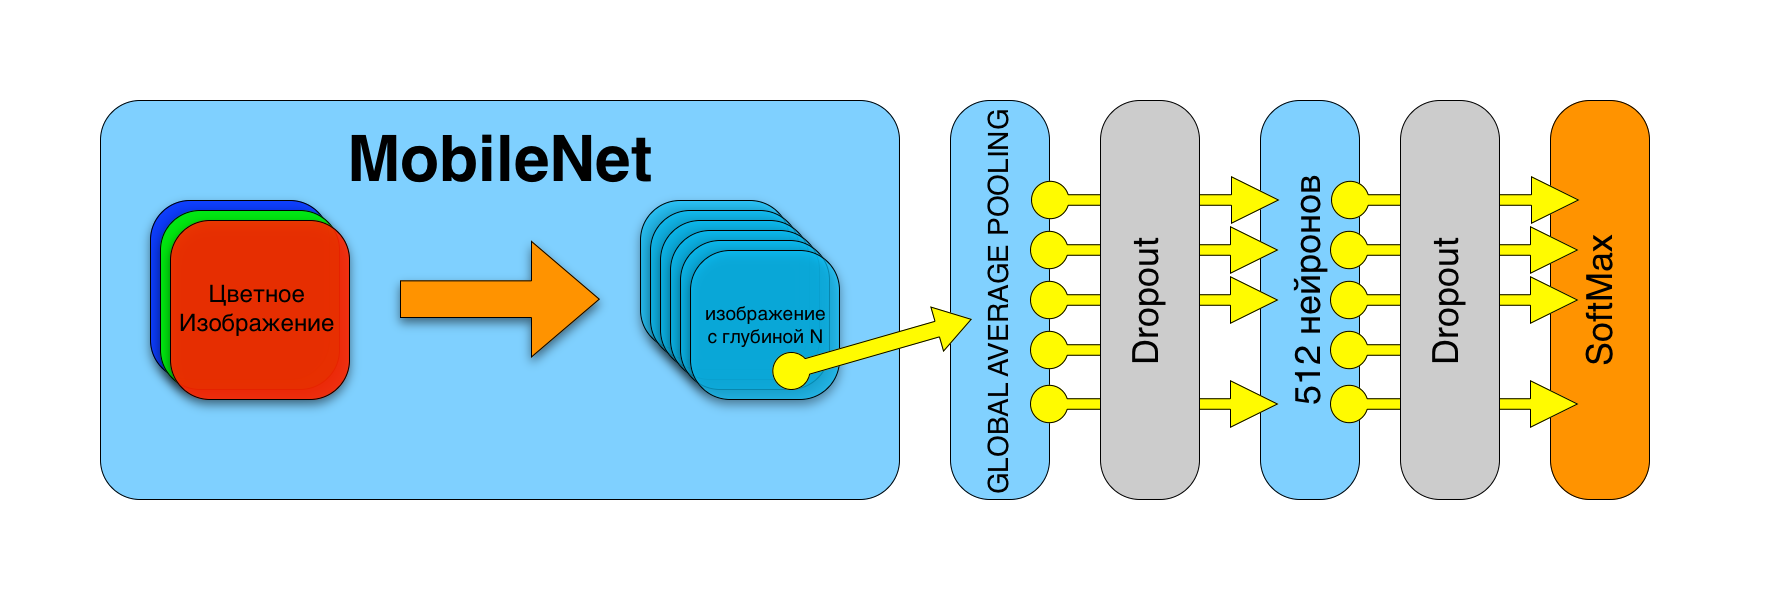
\includegraphics [width=\textwidth] {NN_arch}
  \caption{Архитектура используемой нейронной сети} 
  \label{img:NN_arch}  
\end{figure}


Такая архитектура отлично борется с переобучением нейронной сети на маленьких объёмах данных. Размер входного изображения удерживается на минимальном уровне - 96 пикселей.

Множественные DropOut и Batch Normalization тоже сильно мешают нейронной сети "зазубрить" датасет, так как они каждый раз немного изменяют выходы предыдущих слоёв.

В результате получилась модель, которая с 96\%  точностью на тестовой выборке классифицировала этот датасет. Благодаря мерам по регуляризации, точность на отдельной выборке данных была схожа с точностью на обучающих данных.

\begin{figure}[ht] 
  \center
  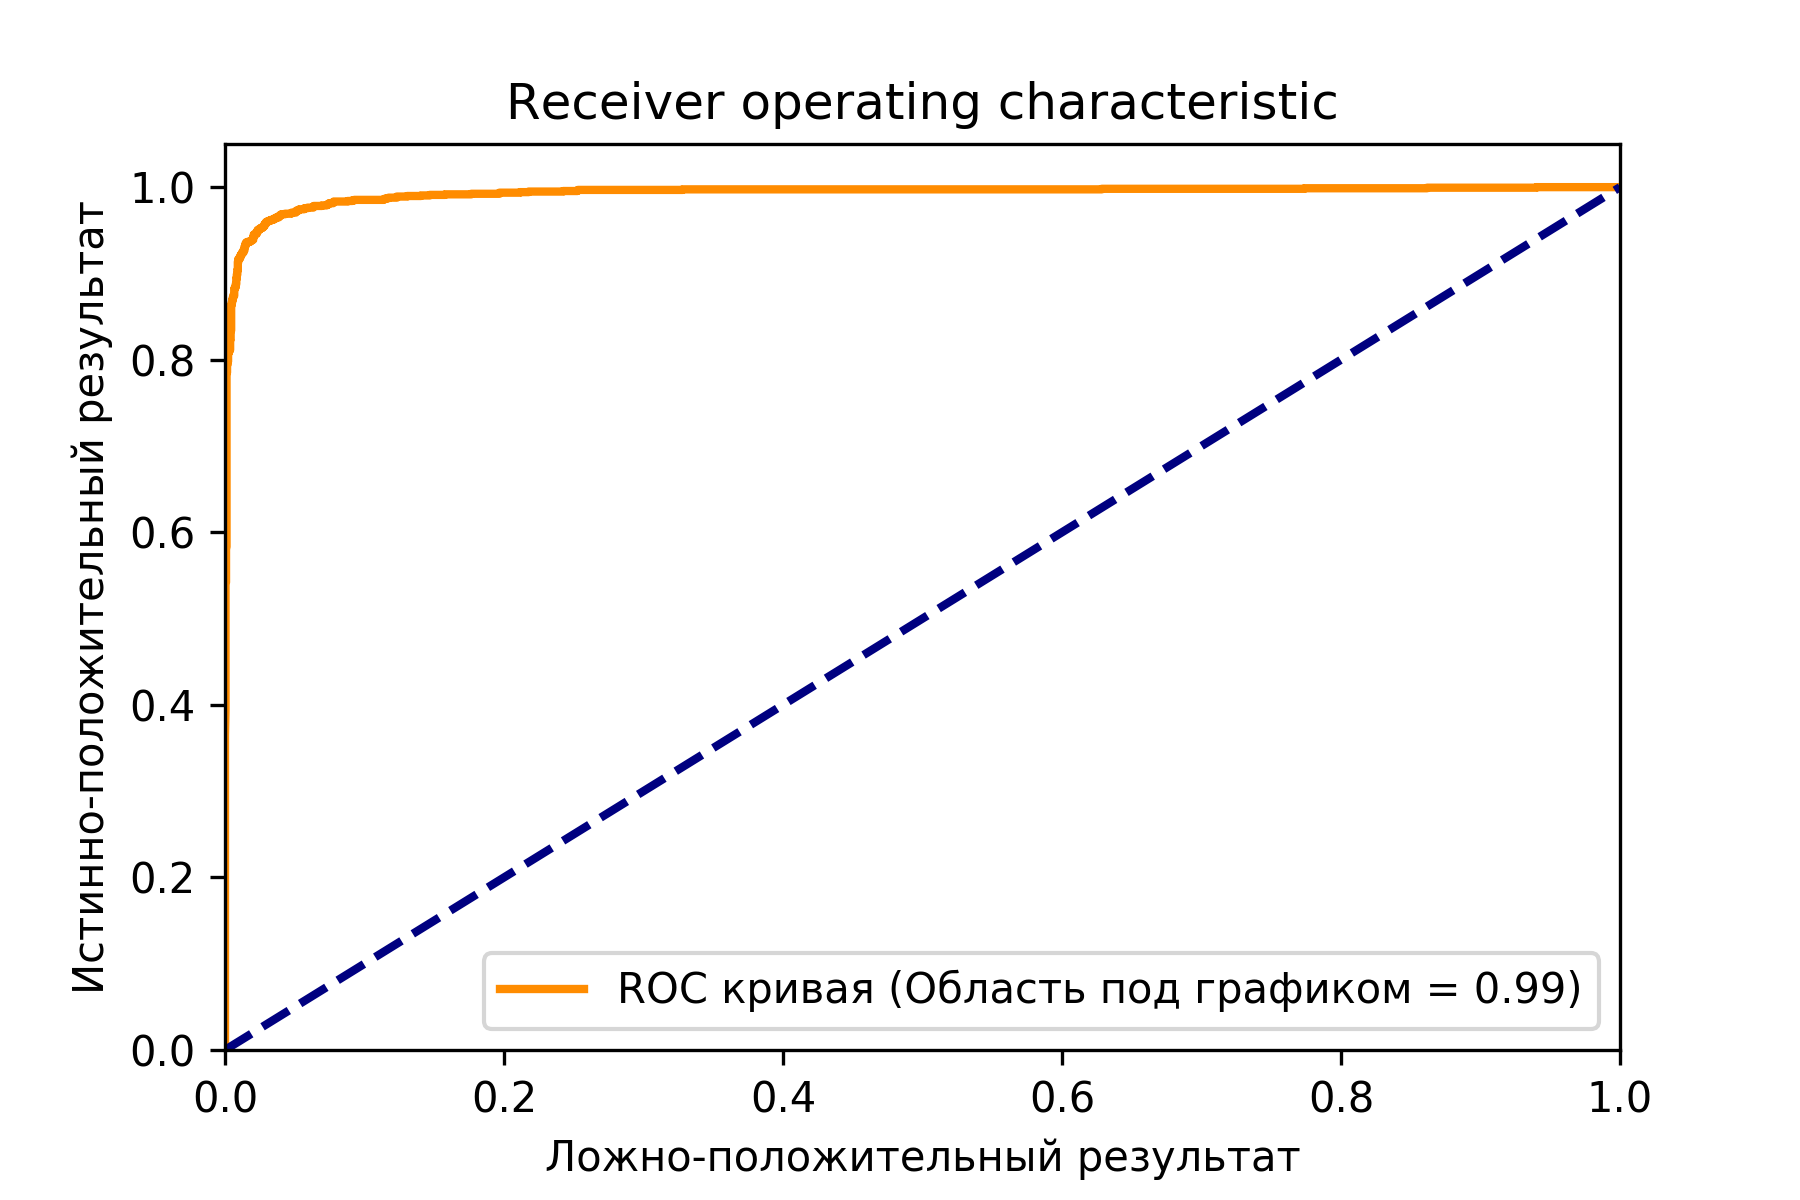
\includegraphics [width=\textwidth*2/3] {ROC_curve}
  \caption{Характеристическая кривая нового классификатора. Чем дальше рыжая кривая лежит от пунктирной линии, тем лучше} 
  \label{img:ROC_curve}  
\end{figure}


\subsection{Оценка качества} \label{quality}
Для оценки качества модели датасет был разделён на три части: 
\begin{enumerate}
    \item Тестовая выборка - 300 изображений;
    \item Валидационная выборка - 100 изображений;
    \item Обучающая выборка - все остальные изображения.
\end{enumerate}

Это делается для того, чтобы при обучении отслеживать насколько модель переобучилась, т.е. зазубрила изображения. Валидационная выборка нужна для того чтобы отслеживать качество модели на каждой эпохе обучения. Тестовая чтобы оценить качество работы классификатора после обучения.

В результате обучения, было получены результаты качества на тестовой выборке, указанные в таблице \ref{tab:classification_report}. Матрица ошибок в нормализованном виде показана на таблице \ref{tab:confusion_matrix}. Характеристическая кривая классификатора показана на рисунке \ref{img:ROC_curve}.

\begin{table}
    \centering
    \captionsetup{justification=centering}
    \caption{\label{tab:classification_report} Отчёт о классификации}
    \begin{tabularx}{\textwidth}{ | Y | Y Y Y | Y |} \hline
           & Точность &  Полнота & f1-score & Количество данных \\\hline

       ЛЕЖИТ  &    0.95  &    0.95  &    0.95  &    114 \\
       СИДИТ  &    0.92  &    0.91  &    0.92  &    93 \\
       СТОИТ  &    0.94  &    0.95  &    0.94  &    93 \\\hline
   Среднее    &  94\% &  94\% &  94\% &  300  \\
 Взвешенное   &  94\% &  94\% &  94\% &  300  \\\hline
    \end{tabularx}
\end{table}


\begin{table}
    \centering
    \captionsetup{justification=centering}
    \caption{\label{tab:confusion_matrix} Нормализованная матрица ошибок. По горизонтали указан истинный класс, а по вертикали предсказанный.}
    \begin{tabularx}{\textwidth}{| Y | Y | Y | Y |}\hline
            & ЛЕЖИТ & СИДИТ & СТОИТ \\\hline
    Лежит   & 0.92 & 0.02 & 0.06 \\
    Сидит   & 0.07 & 0.90 & 0.03 \\
    Стоит   & 0.02 & 0.04 & 0.94 \\\hline
    \end{tabularx}
\end{table}



\section{Разработка приложения}

От приложения требуется определить, присутствует ли на кадре собака и вернуть информацию о позе собаки в данный момент среди следующих классов $Y \in$ (\emph{Стоит,  Сидит,  Лежит}).
\begin{figure}[ht] 
  \center
  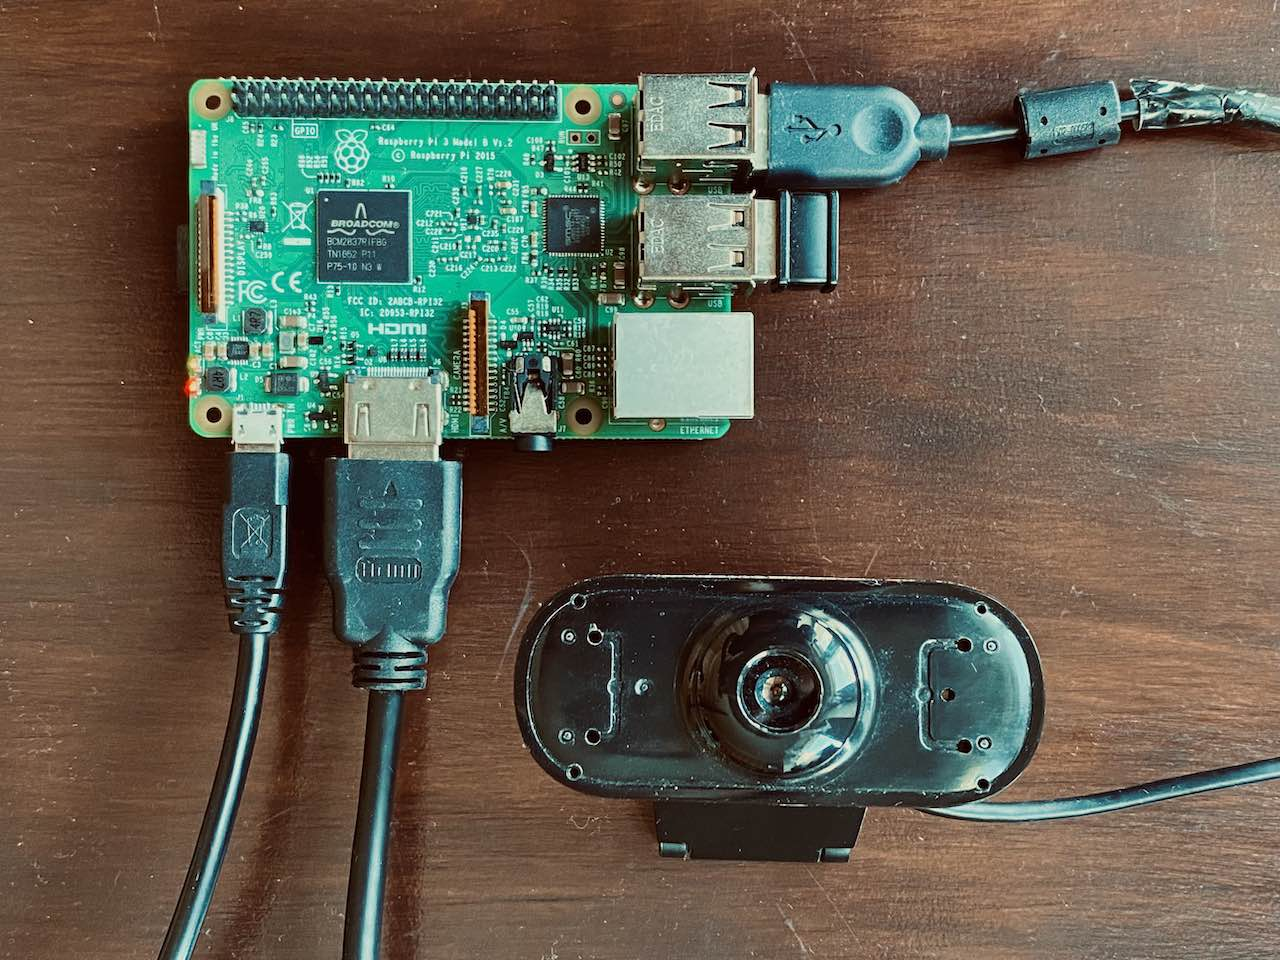
\includegraphics [width=\textwidth*2/3] {target_device}
  \caption{Макет конечного устройства. В нижнем правом углу видна камера устройства.} 
  \label{img:target_device}  
\end{figure}
Как показано на рисунке \ref{img:flowchart}, результирующее приложение получает на вход кадры с изображения и в режиме реального времени камера отслеживает положение собаки если она присутствует в кадре. Далее изображение обрезается по ограничивающей рамке собаки с дополнительным зазором в 15 пикселей чтобы запечатлеть собаку целиком. Информация о локации собаки в кадре и её поза сохраненяются в базу данных. Так как камера стационарна, статистика по локации собаки в кадре должна показать двигалась ли собака по комнате, в которой расположено устройство. 
\begin{figure}[H] 
  \center
  \includegraphics [width=\textwidth*2/3] {flowchart}
  \caption{Функциональная схема поставленной задачи} 
  \label{img:flowchart}  
\end{figure}
Так как конечным устройством был выбран микрокомпьютер Raspberry Pi (см. рисунок \ref{img:target_device}), то требования к производительности оказались достаточно жёсткие. Но благодаря изначальному использованию достаточно компактных нейронных сетей, получилось добиться требуемой производительности. Самая тяжёлая модель, которую пришлось поместить на устройство - это нейронная сеть для обнаружения объектов, которая возвращает позицию собаки в кадре. Её достаточно тяжело в принципе запустить на таких устройствах, но с использованием компактных моделей и квантизации вычислений (использование float16 вместо float32), можно добиться производительности в 5 кадров в секунду (FPS). Здесь достаточно популярным выбором является Mobilenet Single Shot Detector (SSD), обученный на датасете COCO \cite{coco_dataset}.  

Так как модель для классификации и для обнаружения объектов используют одну и ту же родительскую сеть - MobileNet, часть их структуры, а именно свёрточная часть нейронной сети может быть объединена друг с другом. 

MobileNet для классификации позы собаки имеет скорость работы около 8 кадров в секунду. С объединёнными свёрточными слоями можно добиться производительности в 3-4 кадра в секунду.

Но пользователю не требуется даже такая скорость работы, так как конечным результатом всё равно является сбор статистике на длинных промежутках времени (часы - дни). Поэтому, чтобы избежать перегревания Raspberry, достаточно запускать весь процесс всего раз в секунду. А полученная статистика сохраняется на облаке для облегчения доступа к данным.

\subsection{Инструменты и средства разработки}\label{ide}
Программное обеспечение алгоритма распознавания позы собаки было реализовано на языке программирование Python с помощью библиотеки компьютерного зрения OpenCV, а также библиотеки для обучения нейронных сетей Tensorflow в интегрированной среде разработки PyCharm.

Python - интерпретируемый язык с динамической типизацией общего назначения. Данный язык программирования поддерживает такие парадигмы программирования, как процедурное программирование, объектно-ориентированное программирование и обобщенное программирование. Также он обеспечивает модульность, обработку исключений, трассировку ошибок, абстракцию данных, объявление классов объектов и лямбда-функции.

OpenCV (англ. Open Source Computer Vision Library, библиотека компьютерного зрения с открытым исходным кодом) — библиотека алгоритмов компьютерного зрения, обработки изображений и численных алгоритмов общего назначения с открытым кодом.

\section*{Выводы по разделу 4}\label{outro_part_4}
\addcontentsline{toc}{section}{Выводы по разделу 4}
В четвёртой главе была разработана нейронная сеть для классификации позы собак, а также была совершена разработка приложения с её использованием. Это приложение позволяет собирать статистику по передвижениям и по позе собаки в разное время суток. В разработке этого приложения были применена техника квантования вычислений, а для обучения нейронной сети было произведёно исследование подходящих архитектур и параметров сети для получения наивысших результатов.